In this chapter, we provide the context that forms the basis of our research. We begin by presenting a broad overview of the study of brain function, before narrowing down to the specific field of task-based functional Magnetic Resonance Imaging (t-fMRI) that will be the main focus of study in this thesis. Here, we describe each of the preprocessing and modelling components of a typical t-fMRI analysis pipeline. Finally, we give an in-depth discussion of the state-of-the-art procedures used for subject- and group-level t-fMRI inference that are of particular relevance to the remaining chapters of this work. 

\pagebreak

\section{The Study of Brain Function}

\begin{figure}[htbp]
\centering
	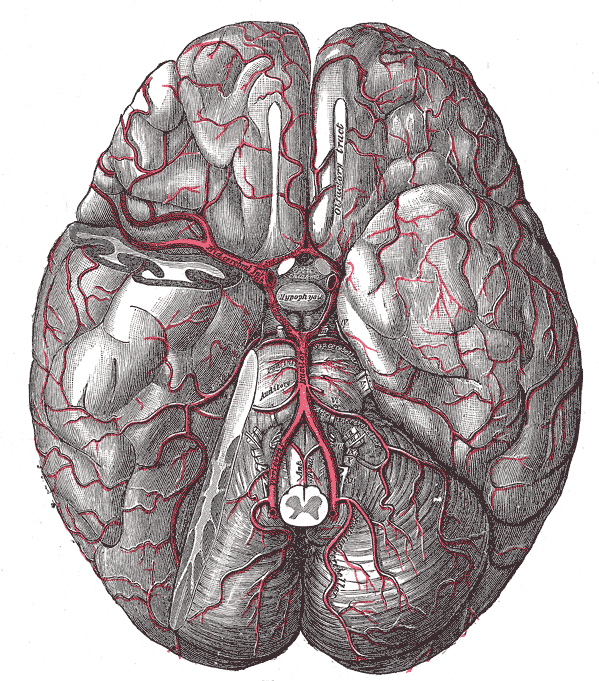
\includegraphics[height=3in]{1_Grays_Anatomy.png}	
\caption*{\textbf{Figure 1:} An illustration showing the arteries at the base of the human brain from (Gray, 1918).}
\end{figure}

The human brain, the central organ of the human nervous system, has been described as one of the most complex structures in the known universe. Made up of approximately 86 billion neurons \citep{Azevedo2009-qj}, where neuronal interaction occurs continuously via trillions of synaptic networks to form intricate and dynamic neural networks, the myriad of processes taking place inside the brain at any given time make the study of brain function an intimidating challenge. Nonetheless, our understanding of this organ has come along way from our ancient Egyptian ancestors, who believed that the heart was at the source of human intelligence, and for whom the practice of drilling a hole into the skull was regarded as a solution to cure a headache \citep{Adelman1987-hs, Mohamed2014-gl}. 

Remarkably, much of this progress has come in the last century alone. A number of key developments within this time-frame include: Confirmation of the neuron doctrine, the concept that the nervous system is a collection of discrete individual cells, postulated by Santiago Ramon y Cajal at the end of the 19th century and demonstrated in the 1950s thanks to the development of electron microscopy \citep{Lopez-Munoz2006-zk}; the first evidence of neuroplasticity, the ability for the brain's structure to change during an individual's lifetime \citep{Diamond1964-cu, Bennett1964-vx}; and the emergence of neuroimaging techniques such as electroencephalography (EEG), positron emission tomography (PET), and MRI. The toils of this scientific endeavour are now translating into concrete advancements influencing a wide variety of aspects concerned with population health. Neuroscience research is beginning to find applications in the clinical setting to advance our understanding of neurodevelopmental and neurodegenerative disorders and generate novel therapies to treat and prevent such diseases. Brain imaging has been used to localize the source of neurological impairment for diseases such as epilepsy \citep{Stacey2008-qx}, and neuroengineering techniques based on our capability to stimulate neural circuits are implemented to treat Parkinson's disease \citep{Kalia2013-bv} and dystonia \citep{Fox2015-ds}. Structural- and functional-MRI are being explored to determine biomarkers for diagnosis of Alzheimer's disease \textit{prior} to symptom onset \citep{Sperling2014-sy, McEvoy2009-zx}, alongside providing information about the role of different brain regions in human behaviour that can contribute to an improved prognosis and patient response to therapy \citep{Matthews2006-sl}.  

Modern neuroscience can be dissected into many major branches, each subfield taking a specific slant to studying the nervous system. It is therefore perhaps unsurprising that in isolation, the phrase `the study of brain function' is rather vague. Brain function can manifest itself in ways that can be observed using a variety of different measurements, whether that be with a molecular, chemical, structural, or functional approach \citep{Hargreaves2012-dz}. Different modalities of MRI are employed to evaluate specific properties that ultimately characterize whichever approach is taken. For instance, looking at brain function from an anatomical perspective, voxel-based morphometry (VBM) could be used to measure differences in local concentrations of brain tissue, to assess, for example, changes in grey matter volume \citep{Mechelli2005-dn}. Additionally, one could apply diffusion tensor imaging (DTI) to instead map white matter tractography in the brain \citep{Alexander2007-ut, Soares2013-mh}. From a functional outlook, resting state fMRI (rs-fMRI) determines that spatially remote brain areas are functionally connected when each region's BOLD response is temporally correlated in the absence of an explicit task \citep{Lee2013-kn}. On the other hand, task-based fMRI (t-fMRI) measures spatio-temporal changes in the BOLD signal between task-stimulated and control states to find brain regions that are activated in the presence of a stimulus \citep{Glover2011-at}. 

Each imaging method and modality does not live inside a vacuum, and recent work within the field has provided further insight of the interdependence between different approaches to examining brain function. One example of this is in the study of resting state networks, which explores how distinct sets of brain regions can reveal temporally correlated activation patterns when the brain is at rest. While resting state networks have been most widely investigated using rs-fMRI techniques \citep[e.g.][]{Smith2009-dm, Lee2012-di, Moussa2012-bl}, more recently, the same correlation patterns have been independently detected using EEG and MEG \citep{Brookes2011-cj, Fomina2015-ha}. This work not only demonstrates how utilization of numerous tools can further our understanding of resting state mechanisms, but also suggests a direct relationship between the electro-physiological signals recorded with MEG and the BOLD fluctuations associated to fMRI. Similarly, other recent efforts have shown that the functional response to a cognitive task measured with t-fMRI may be able to be predicted by connectivity features from the same individual's brain at rest \citep{Parker_Jones2017-ld, Tavor2016-pd}. This research signals towards an innate functional signature that defines our behaviour, while also providing potential clinical solutions to obtain t-fMRI data from patients who are unable to perform the specific task of interest.  

In the context of this thesis, we will study brain function from a functional perspective, primarily focussed on task-based fMRI. 

\section{Blood Oxygenation Level Dependant (BOLD) Functional Magnetic Resonance Imagery (fMRI)}

Whereas structural MRI is concerned with the anatomy of the brain, functional MRI (fMRI) measures dynamic changes in blood flow in order to ultimately make inference on neuronal activation. This is possible due to the intrinsic relationship between local neuronal activity and subsequent changes in cerebral blood flow (CBF), a biological phenomenon known as neurovascular coupling. An increased supply of oxygen is carried by haemoglobin in red blood cells to provide energy to active neurons, and it is the magnetic properties of the haemoglobin that MRI takes advantage of. Specifically, as deoxygenated haemoglobin is more magnetic (paramagnetic) than oxygenated haemoglobin, MRI uses haemoglobin as an endogenous contrast agent from which to source the signal. Neurovascular coupling induces inhomogeneities in the local magnetic field due to a decreased concentration of deoxygenated haemoglobin, that lead to a detectable change in the MR signal.

The complete chain of events linking neuronal activity to a change in MRI signal is referred to as the Blood Oxygenation Level Dependant (BOLD) effect, and this type of imaging is known as BOLD fMRI.  Proof of concept of the BOLD effect was first provided in \citet*{Ogawa1990-it}, and the first use of BOLD fMRI for human brain mapping was carried out in 1992 \citep{Bandettini1992-jt, Kwong1992-uq, Ogawa1992-af}, leading to a large uptake of the method that has continued to this day. Alternative approaches to functional imaging exist, the most popular of which is functional Arterial Spin Labelling (fASL), that uses magnetically labelled arterial blood water to quantify changes in CSF. While fASL can offer some advantages over fMRI, and changes in CSF measured with the technique are more closely tied to neuronal activation than the BOLD signal, fASL suffers from a much lower signal-to-noise ratio that consequently has made fMRI the preferred imaging modality of choice. 

\subsection{Physiology of the BOLD response}

\begin{figure}[htbp]
\centering
	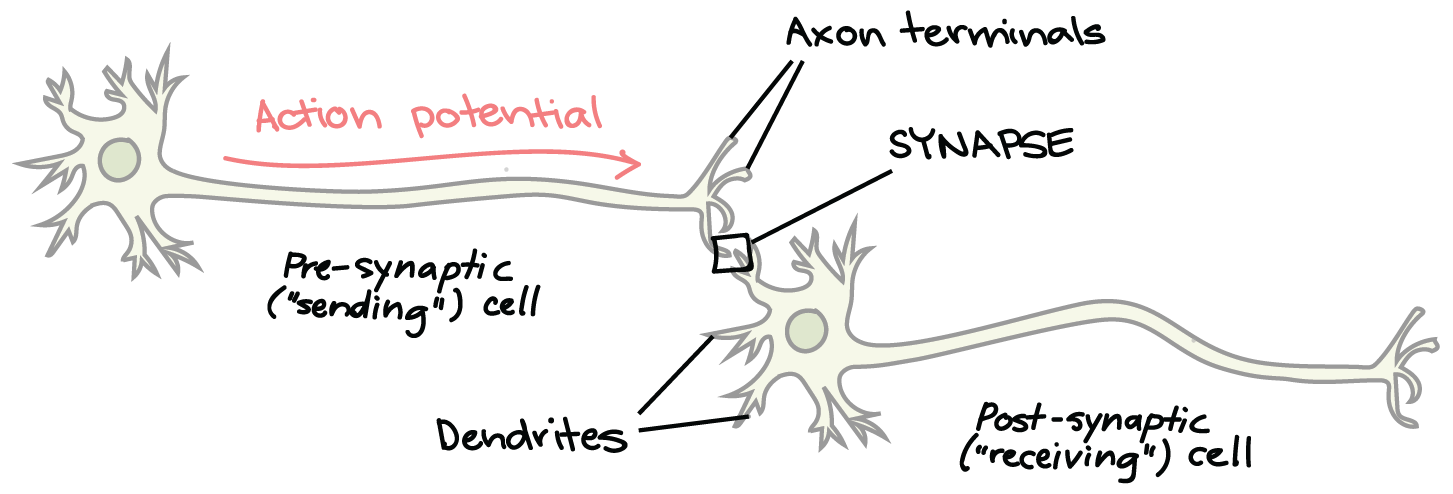
\includegraphics{2_Neuron.png}	
\caption*{\textbf{Figure 2:} A schematic of the interaction between neurons. Image reused from Khan Academy (\href{https://creativecommons.org/licenses/by-nc-sa/3.0/us/}{CC BY-NC-SA 3.0 US}). Note: All Khan Academy content is available for free at (\href{https://www.khanacademy.org/}{www.khanacademy.org}).}
\end{figure}

Neuronal interaction transpires via a system of electrical and chemical activity. To send out information, an individual neuron -- the pre-synaptic cell -- emits an electrical signal known as an action potential, for the purpose of stimulating another target neuron -- the post-synaptic cell. The action potential travels along the axon of the sending cell, and is transmitted to the receiving cell at the synapse. Information is delivered from the output branches (or, \textit{axon terminals}) of the sending cell across the synapse to the input branches (or, \textit{dendrites}) of the receiving cell, involving the release of chemical \textit{neurotransmitters} alongside a number of other cellular processes. This may stimulate or inhibit the firing of action potentials at the target cell to communicate with other neurons, eventually leading to a configuration of neurons collectively processing and responding to information. 

The electrical and chemical processes involved in neuronal activation require energy, which drives the neurovascular coupling. Blood vessels that flow into the capillaries pervading the neuronal tissue dilate and the rate of CBF increases to regulate a greater supply of oxygen and nutrients to localized regions of active neurons. Overall, the increases in CBF and cerebral blood volume (CBV) are many orders of magnitude greater than the increases in oxygen extraction (CMRO$_{2}$) caused by the neuronal activation. Thus, there is an overall net increase of oxygenated heamoglobin, and an increase in the BOLD signal. The expected BOLD response generated from a brief stimulus is characterized quantitatively by the Hemodynamic Response Function (HRF), encompassing the individual changes in CBF, CBV and CMRO$_{2}$ induced by neuronal stimulation. 

\begin{figure}[htbp]
\centering
	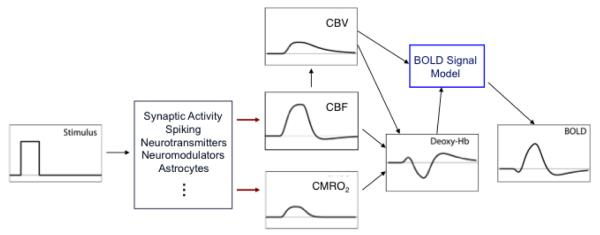
\includegraphics{3_BOLD_response.jpg}	
\caption*{\textbf{Figure 3:} Blah}
\end{figure}


\section{Task-based functional Magnetic Resonance Imagery (t-fMRI)} 
\label{sec:t-fMRI}

The ultimate goal of a task-based functional Magnetic Resonance Imagery (t-fMRI) experiment is to understand the brain regions that are responsive to a particular task or stimulus the researcher has chosen to investigate. Explicitly, the researcher seeks to detect brain areas whose BOLD time series data is correlated to the task the participant is instructed to perform in the scanner. Researchers can choose from a wide range of possible tasks to explore how the brain processes in a variety of circumstances. For example, a cognitive task may be chosen to gain insight into how the brain processes decision-making or recognition, while a physiological task may be used to see how the brain reacts to a stimulus intended to cause pain or arousal, or how the brain functions when participants are told to hold their breath. In general, the experimenter is only limited in choice of task by the constraints that the task must be able to be conducted within the scanner, and that the task should not involve any sort of head movement which could corrupt the signal. 

The MR signal measured in the scanner is noisy, and the heamodynamic response induced by a stimulus only causes fractional changes in the BOLD response, typically of around one percent. Therefore, in order to increase the signal-to-noise ratio (SNR) of the BOLD signal participants repeat the task several times in the scanner. The type of task used, alongside the timings for which the participant is instructed to perform the task inside the scanner, are together known as the \textit{task paradigm} or \textit{experimental design}. Many different task conditions can be investigated within one task paradigm, however, it is fundamental that at least two conditions are included. This is because BOLD data are not quantitative, insofar that we are unable to interpret the level of neuronal activity from the absolute magnitude of the BOLD response alone. Instead, neuronal activity is inferred by using \textit{contrasts} to measure the difference in the MR signal between two conditions. Commonly, the BOLD response to a task condition is contrasted with a \textit{baseline} condition, where the participant is at rest within the scanner. However, it is equally acceptable to contrast two separate task conditions depending on the aims of the investigation. 

An experimental design where the task condition is carried out for an extended period of time is said to have a \textit{block} design (or \textit{boxcar} design). One example of this could be a task paradigm where the participant is instructed to look at an animal photo for five seconds in each task repetition. Alternatively, in an \textit{event-related} design the task or stimulus takes the form of a discrete, rapid event, such as a study where the participant experiences a mild electric shock. A graphical representation of each of these task paradigms is shown in \textit{Figure BLAH}, along with the anticipated response from each type of stimulus. While block designs have greater statistical power, with a relatively larger BOLD response, the researcher has more control with respect to how the stimuli are delivered in an event-related design. 

\begin{figure}[htbp]
\centering
	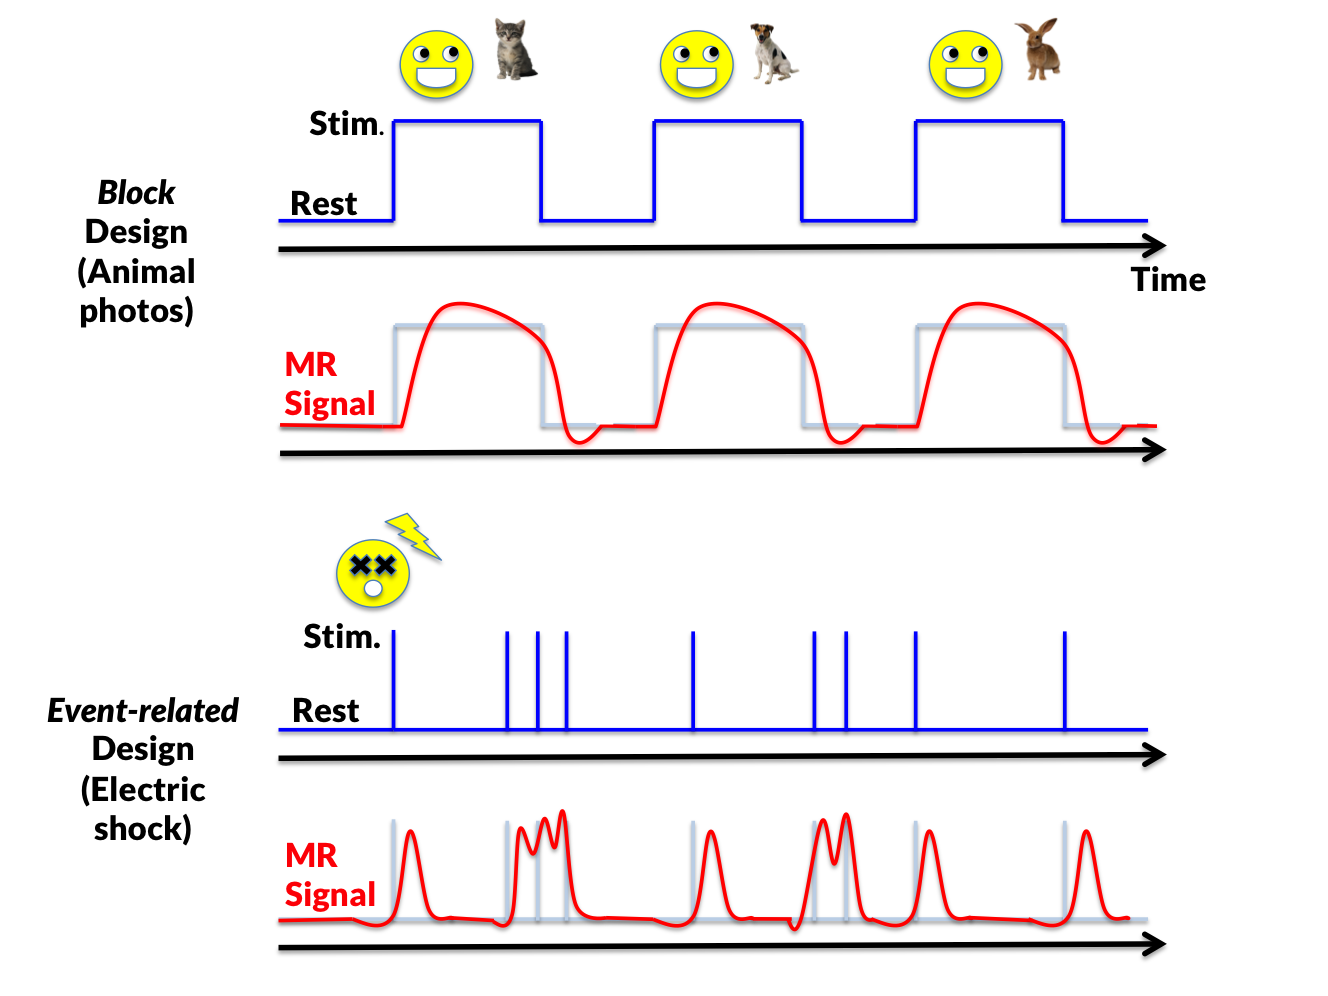
\includegraphics[height=4.0in]{4_Task_Paradigm.png}
\caption*{\textbf{Figure 4:} Blah}
\end{figure}

\section{Overview of Analysis Pipeline}

To analyse voxelwise t-fMRI BOLD data, a series of analysis steps are performed on the data in succession. Together, the complete chain of analysis procedures carried out is known as the analysis \textit{pipeline}. Researchers have great flexibility as to how the analysis pipeline is comprised, with various options and adjustable parameters for each individual analysis step, as well as choices as to the order in which certain procedures are conducted. Nevertheless, a standard analysis pipeline of t-fMRI data can be partitioned into three main stages: preprocessing, modelling, and statistical inference. In the upcoming sections we will describe the individual processing steps that are usually carried out in each of these analysis stages, while here we provide a brief overview.

The main goals of preprocessing are to reduce the severity of noise artefacts present in the raw BOLD fMRI data, and to prepare the data for statistical analysis. At the modelling stage, a mass-univariate approach is adopted, whereby each voxel's functional time series data is considered independently as an instance of the general linear model (GLM) framework. Within the GLM, the contrasts discussed in the previous section are formulated to statistically test the main hypotheses investigated within the study. At the inference stage, a \textit{statistical parametric map} is generated containing statistic values at each voxel for each contrast of interest. For \textit{subject-level} inference, a participant's statistical parametric map is thresholded to display only voxels showing statistically significant results. This type of inference may be of interest in a clinical setting, particularly to aid in the diagnosis of a patient, however in a research study there is usually a greater emphasis placed on finding results that generalize across the larger population. In this case, each participant's statistic map is entered into a second-level model for \textit{group-level} inference, and a thresholded map is computed to localize effects that were consistent across all individuals in the study. 


In practice, the analysis pipeline is usually carried out within a neuroimaging \textit{software package}. Various software packages are available, many of which are freely distributed on the internet. The three most popular packages are \textit{AFNI} \citep{Cox1996-nu}, \textit{FSL} \citep{Jenkinson2012-wh}, and \textit{SPM} \citep{Penny2011-uk}. While there are several differences as to how each software package operates, most packages follow the same fundamental principles to implement the three main stages of the analysis pipeline.     


\section{Preprocessing}

In this section, we present each of the analysis steps that are typically conducted within a t-fMRI preprocessing pipeline: brain extraction, distortion correction, slice-timing correction, realignment, coregistration, spatial normalization, spatial smoothing, temporal filtering and intensity normalization. These procedures are carried out to compensate for artefacts present in the data, and to ensure that the data satisfy the assumptions used for modelling and inference. 

\subsection{Brain Extraction}

\textit{Brain extraction} is commonly the first procedure carried out in the analysis pipeline, with the purpose of removing the skull and any other non-brain tissue from a participant's anatomical image. Since the purpose of the analysis is to infer areas of activation \textit{within} the brain, conceptually it is sensible to remove any external structures that are not of interest. However, brain extraction also has a more important role in improving the outcome of subsequent steps in the preprocessing pipeline. In the upcoming sections we describe \textit{coregistration}, where the subject's functional data is spatially realigned to the anatomical image, as well as \textit{spatial normalization}, where each participant's data is registered to a standard space. Brain extraction helps to increase the robustness of both of these registration methods, since differences in non-brain structures can sidetrack the registration algorithms causing an inaccurate alignment of the respective images. 

In SPM, brain extraction is carried out by first applying a \textit{segmentation} to the anatomical image, in order to generate probability maps of the gray and white matter tissue in the structural scan. The grey and white matter probability maps are summed and thresholded, creating a binary map containing the brain regions to be included in the analysis. Finally, the anatomical scan is masked with the binary map to remove any non-brain structures. AFNI and FSL both use variants of the Brain Extraction Tool \citep{Smith2002-vw} algorithm, implementing an adaptive model that evolves to fit the brain's surface in order to segment brain and non-brain tissue types. 

\subsection{Distortion Correction}

\textit{Distortion correction} is applied to account for signal loss and geometric distortions in the functional data that can manifest due to spatial inhomogeneities in the main static magnetic field during the acquisition. These inhomogeneities arise due to the different magnetic susceptibility properties of each tissue type in the brain, and the most severely affected regions are those close to air-filled synuses, such as the temporal or frontal lobe. If not corrected, signal dropout and distortion can cause failure in the registration of the functional data to the non-distorted anatomical image. 

While it is not possible to recover regions of signal loss, field distortions can be rectified with the use of a \textit{field map}. A field map is obtained as part of the acquisition to estimate the intensity of the static magnetic field. The analysis software uses the field map to calculate the magnitude of the geometric distortions, and then applies spatial transformations to unwarp the functional data.  The field map is also used to deweight areas of substantial signal dropout during the registration, and if the signal loss is particularly severe, ignore these locations in the analysis of the data. 

\subsection{Slice timing Correction}

While the statistical modelling of fMRI data assumes that the signal is measured over the entire brain simultaneously, in reality functional imaging is usually carried out on a slice-by-slice basis, creating a single 3D volume as a combination of multiple 2D slices. Slices are acquired sequentially from top-to-bottom or bottom-to-top, or by using an interleaved sequence where all odd-numbered slices are collected first, followed by the even slices. Because of this, the BOLD signal is sampled at different points of the HRF. This can create the illusion that the signal peaks earlier for slices that are collected later in the acquisition, even though the underlying response is identical. 

\textit{Slice timing correction} uses temporal interpolation methods to artificially obtain an intensity estimate at each brain voxel at a single time point, shifting the data to recreate the image as if all measurements were obtained collectively. The reference time point is commonly chosen to be halfway through the scanning procedure, and in this case the timings from all slices are corrected to match-up with the timings of the volume collected midway in the acquisition, which acts as the reference slice. The time series data from each voxel is temporally shifted to line-up with the signal response from the reference slice, and the voxel's data between the acquisition time points of the reference slice are re-estimated with interpolation. Commonly, this is done using either sinc or spline interpolation. 

It is debatable whether slice timing correction should be conducted before or after realignment, and some practitioners have suggested that slice timing correction should be excluded from the analysis pipeline altogether. One alternative to slice timing correction is to account for timing differences at the modelling stage of the analysis. FSL recommend that temporal derivatives are incorporated as extra regressors into the GLM, effectively making the model flexible to temporal shifts in the signal response. 

\subsection{Realignment}

While a participant is told to remain as still as possible in the scanner, over the course of the acquisition some head movement is inevitable. This is particularly problematic in fMRI, as it can corrupt the functional data in numerous ways. If left uncorrected, head movement may cause a voxel's time series data to contain signal from two different tissue types, and if the voxel is located at the edge of the brain, may lead to a loss of signal altogether. Additionally, the change in signal intensity induced by head motion can be many orders of magnitude greater than the BOLD effect. Therefore, if head motion is elicited by the task the participant performs in the scanner, this can lead to false activations in the statistical results that invalidate the analysis. 

\textit{Realignment} (or \textit{motion correction}) of the functional data is performed to remove any substantial movement throughout the time series. To do this, each volume in the time series is spatially transformed to match a reference volume, usually chosen as the first volume of the data or an average image of all the scans. Specifically, a rigid-body transformation of translations and rotations is applied to superimpose each volume onto the reference image. The transformation is determined to optimize a cost function that quantifies the goodness of alignment between the images, e.g. a least squares (used by default in SPM) or normalised correlation (used by default in FSL) cost function. Finally, the transformed data are spatially interpolated to obtain estimates of the signal response on the same voxel grid as the reference image, usually with spline interpolation.

\subsection{Coregistration}

In order to carry out group analyses, corresponding voxels between each participant's functional data should contain information from the same physical anatomical location. However, prior to normalizing data \textit{between} subjects, \textit{coregistration} is conducted to align a participant's functional time series data with their own anatomical image. Similar to realignment, coregistration is achieved via a rigid-body transformation chosen to minimize an appropriate cost function. However, to account for differences between the blurry, distorted functional data and the high-resolution structural image, scalings are also included as parameters of the rigid-body transformation, and a mutual information cost function is commonly used.    

\subsection{Spatial Normalization}

The goal of \textit{spatial normalization} (or \textit{intersubject registration}) is to warp all participants functional time series data into a universal coordinate space, integrating the data between subjects to facilitate for group analyses. To remove structural variability between subjects, each participant's data is spatially transformed onto a standard template brain image. The most commonly used templates are the MNI152 images, created by the Montreal Neurological Institute by combining structural data from 152 healthy adults. The transformation is computed on a participant's structural image; the anatomy is registered to the template with a series of linear and non-linear transformations, permitting for local deformations to change the size and shape of the subject's structural image for a better alignment with the brain standard. Finally, the functional data are warped to standard space by concatenating the transformation from functional to structural space computed during coregistration with this transformation from structural to standard space. 

\subsection{Spatial Smoothing}

Prior to statistical analyses, \textit{spatial smoothing} is conducted on the functional data. Although this step may seem unsound, as any smoothing will effectively reduce some of the spatial resolution of the fMRI data, the reasons for spatial smoothing are twofold. First and foremost, the  main reason for smoothing is to improve the SNR of the data by filtering out high-frequency regions. Intuitively, this works because averaging should reduce the intensity of noisey areas, while leaving the underlying functional signal of interest relatively unaffected. The second reason for smoothing is as a prerequisite for statistical analysis. Specifically, the Gaussian random field theory used for parametric inference is adaptive in how it corrects for the multiple comparison problem dependant on the smoothness of the data. However, a minimum amount of smoothing is required to obtain accurate control over the false discovery rate of activations in the thresholded statistical results.

In practise, the functional data are convolved with a three-dimensional Gaussian filter, and the amount of smoothing applied is proportional to the full width at half maximum (FWHM) of the kernel function. A suitable degree of smoothing is conditional on many factors, such as the quality of the data, the statistical power required, and the expected size of the final activation clusters. A typical smoothing kernel FWHM is between 6 and 10mm$^{3}$, although the preprocessing pipelines for recent high-quality, large-sample fMRI datasets have used a lesser degree of smoothing (e.g. 5mm FWHM for the UK Biobank, 4mm FWHM for the Human Connectome Project). 
 

\subsection{Temporal Filtering}
\label{sec:temporal_filtering}

\textit{Temporal filtering} is another processing step that aims to increase the SNR of the functional data, by taking advantage of the fact that the BOLD signals fMRI sets out to measure generally have a consistent frequency range. Temporal filtering suppresses or removes frequencies outside of this range, implicitly eliminating any artefactual signals present in the data while leaving the neuronal signals of interest untouched.

A well-known source of noise is slow drifts that occur due to imperfections in the scanning hardware. As components of the scanner heat up, this can induce a gradual change in the MR signal resulting in low frequency trends of less than 0.01 Hz in the data. The expected frequency of the BOLD signal response to a task stimulus is around 0.2Hz. Therefore, a \textit{high-pass filter} can be applied, removing all frequencies below a set threshold to attenuate scanner-related drifts. Other forms of noise are caused by physiological effects such as respiratory and cardiac cycles. These artefacts have a frequency range higher than the expected BOLD response (respiratory frequencies are $\sim$0.3hz, cardiac frequencies $\sim$1.0hz), although they may also manifest in the data as lower frequencies due to the effects of \textit{aliasing}. A \textit{low-pass filter} may be used to cut off higher frequencies and subdue artefacts such as physiological noise. While a high-pass filter is commonly included as part of the preprocessing pipeline, low-pass filters are more controversial as they can cultivate autocorrelation in the signal, violating the assumption of temporal independence made for statistical inference. 

\subsection{Grand Mean Scaling}

As touched on in \textit{\ref{sec:t-fMRI}}, BOLD t-fMRI data are not quantitative. Because of this, the fMRI scanner assigns arbitrary units to the signal intensities during the acquisition, and data can be scaled differently across scanning sessions. \textit{Grand mean scaling} (or \textit{intensity normalization}) is applied to rescale each individual's functional time series to increase the interpretability of the data across the group of participants. This is done by multiplying the functional time series (across all voxels and time points) by a constant so that the mean intensity takes a fixed value of, for example, 100. While grand mean scaling will not affect the statistical inference results, normalizing the data facilitates for comparability of the regression coefficient maps (i.e. \textit{beta} maps) obtained for each task condition at the modelling stage of analysis.  

\section{Modelling of t-fMRI data with the General Linear Model}

The \textit{General Linear Model} (GLM) is the most widely used approach to modelling BOLD t-fMRI time series data, and a crucial part of any neuroimaging analysis. The GLM generalises a broad class of models that estimate the observed response as a linear combination of experimental and confounding variables. A key strength of this framework is its flexibility, allowing for analyses of data both within and between individuals, and providing a foundation for which experimental hypotheses can be assessed with a variety of statistical tests, using either parametric or nonparametric statistics. In this section we provide an overview of the GLM in the context of brain imaging, before describing some of the most commonly used statistical tests performed within the GLM for analysing fMRI data.


\subsection{The GLM Set-up}
\label{sec:GLM}
To analyse voxelwise t-fMRI data, each voxel's time series is independently modelled within the GLM. This is commonly referred to as a \textit{mass-univariate} analysis -- the `mass' term specifies that the same analysis is performed many times, and `univariate' indicates that each analysis is performed separately at every brain voxel (as opposed to \textit{multivariate}, which considers many locations as part of one analysis). 

Mathematically, for a compact domain $S \subset \mathcal{R}^{D}$ (in fMRI, $D$ = 3 and $S$ is the brain mask), the GLM at location (or brain voxel) $\bm{s} \in S$ is expressed as
\begin{equation}
\label{eq:GLM}
\bm{Y}(\bm{s}) = \bm{X}\bm{\beta}(\bm{s}) + \bm{\epsilon}(\bm{s}),
\end{equation}
where $\bm{Y}(\bm{s})$ is an $N \times 1$ vector of observations at $\bm{s}$, $\bm{X}$ is an $N \times p$ design matrix containing explanatory variables linking the observations in $\bm{Y}(\bm{s})$ to the effect sizes in $\bm{\beta}(\bm{s})$, $\bm{\beta}(\bm{s})$ is an $p \times 1$ vector of the unknown parameters, and $\bm{\epsilon}(\bm{s})$ is an $N \times 1$ vector of error terms. It is assumed that the errors are independently distributed conditional on $\bm{X}$ by a Gaussian distribution with mean zero.

The aim of the regression is to find parameter estimates $\bm{\hat{\beta}}(\bm{s})$ that best fit the model to the data. The goodness of fit is determined by a method of \textit{least squares}, depending on additional constraints added to the model. The parameter estimates are then used at the inference stage to test hypotheses about the data expressed in terms of the unknown parameters contained in $\bm{\beta}(\bm{s})$.

\subsection{Estimating the Parameters with Ordinary Least Squares (OLS)} 

OLS is used to solve \ref{eq:GLM} with the assumption that the errors are \textit{spherical}, which means that there is no autocorrelation and that each error term has constant variance. Combined with the normality assumption stated in the previous section, this means
\begin{equation}
\label{eq:OLS_errors}
\bm{\epsilon}(\bm{s}) \mid \bm{X} \sim  \mathcal{N}(0, \sigma^{2}(\bm{s})\bm{I}_{N}),
\end{equation}
where $\bm{I}_{N}$ is the $N \times N$ identity matrix. OLS solves the GLM by minimizing the \textit{sum of squares} cost function $S$ given by
\begin{equation}
\label{eq:OLS_cost}
S(\bm{\beta}(s))  = \lVert \bm{Y}(\bm{s}) - \bm{X}\bm{\beta}(\bm{s}) \rVert^{2} = \sum_{i = 1}^{N} \lvert Y_i(\bm{s}) - \sum_{j = 1}^{p} X_{ij} \beta_j (\bm{s}) \rvert ^{2}.
\end{equation}
This gives the OLS estimates
\begin{equation}
\label{eq:OLS_estimates}
\hat{\bm{\beta}}(\bm{s}) = \argmin_{\bm{\beta}} S(\bm{\beta}(\bm{s})) = (\bm{X}^{\intercal}\bm{X})^{-1}\bm{X}^{\intercal}\bm{Y}(\bm{s}).
\end{equation}
By the Gauss-Markov Theorem, it can be shown that the OLS estimates are the Best Linear Unbiased Estimates (BLUE) of $\bm{\beta}(\bm{s})$ providing all the assumptions are satisfied. 

\subsection{Prewhitening}

The key assumption of OLS is that the errors are spherical, however, this is often violated for fMRI data. As discussed in \ref{sec:temporal_filtering}, functional data are characterized by slow drifts which induce temporal autocorrelation in the MR signal. While high-pass filtering can be applied in an attempt to remove the majority of low frequency components, another strategy is to estimate the autocorrelation directly and then remove it by \textit{prewhitening} the data. This can be more efficient than filtering for event-related designs (Woolrich, Temporal Autocorrelation in Univariate ...).

If the data are correlated, the error terms have marginal distribution 
\begin{equation}
\label{eq:correlated_errors}
\bm{\epsilon}(\bm{s}) \mid \bm{X} \sim  \mathcal{N}(0, \sigma^{2}(\bm{s})\bm{V}(\bm{s})),
\end{equation}
where $\bm{V}(\bm{s})$ is the correlation matrix. Since $\bm{V}(\bm{s})$ is symmetric and positive-definite, $\bm{V}(\bm{s})$ satisfies the assumptions for the Cholesky decomposition, which means there exists a lower triangular matrix $\bm{K}(\bm{s})$ such that $\bm{V}^{-1}(\bm{s}) = \bm{K}^{\intercal}(\bm{s})\bm{K}(\bm{s})$. Providing that $\bm{K}(\bm{s})$ can be accurately determined, the idea is to update the model by multiplying both sides of the GLM by $\bm{K}(\bm{s})$ so that the error terms are spherical. Denoting $\bm{Y}^{*}(\bm{s}) = \bm{K}(\bm{s})\bm{Y}(\bm{s})$, and defining $\bm{X}^{*}(\bm{s})$ and $\bm{\epsilon}^{*}(\bm{s})$ similarly, then for the updated GLM
\begin{equation}
\label{eq:updated_GLM}
\bm{Y}^{*}(\bm{s}) = \bm{X}^{*}(\bm{s}) + \bm{\epsilon}^{*}(\bm{s}),
\end{equation}
the conditional covariance of $\bm{\epsilon}^{*}(\bm{s})$ is
\begin{equation}
\label{eq:updated_error_cov}
\mathrm{Cov}(\bm{\epsilon}^{*}(\bm{s}) \mid \bm{X}) = \bm{K}(\bm{s})\mathrm{Cov}(\bm{\epsilon}(\bm{s}) \mid \bm{X})\bm{K}^{\intercal}(\bm{s}) = \sigma^{2}(\bm{s})\bm{I}_{N}.
\end{equation}
Therefore, the sphericity assumption is satisfied for the updated model, and OLS can be applied to obtain the BLUE of $\bm{\beta}(\bm{s})$.

\subsection{Estimating the Variance}
For statistical inference, the variance of the errors $\sigma^{2}(\bm{s})$ needs to be estimated. This can be done using the OLS estimates. The \textit{fitted values} given by the OLS estimates are $\hat{\bm{Y}}(\bm{s}) = \bm{X}\hat{\bm{\beta}}(\bm{s})$. The differences between the observed data points and the fitted values are known as the \textit{residuals}, denoted by $\hat{\bm{\epsilon}}(\bm{s}) = \bm{Y}(\bm{s}) - \hat{\bm{Y}}(\bm{s})$. The variance of the errors is estimated as the sum of squares of the residuals divided by the \textit{degrees of freedom} of the model
\begin{equation}
\label{eq:variance_estimator}
\hat{\sigma}^{2}(\bm{s}) = \frac{\bm{\epsilon^{\intercal}}(\bm{s})\bm{\epsilon}(\bm{s})}{N - p};
\end{equation}
The degrees of freedom are $N - p$, since there are N observations $Y_{1}(\bm{s}), ..., Y_{N}(\bm{s})$, and $p$ parameters $\beta_{1}(\bm{s}), ... , \beta_{p}(\bm{s})$ to estimate.

\subsection{Inference with Null-Hypothesis Significance Testing}
The pay off from obtaining the parameter estimates using OLS is that it enables us to statistically test hypotheses about the unknown effect sizes. This form of inference is known as \textit{Null-Hypothesis Significance Testing}. Hypotheses are expressed using a contrast vector $\bm{c}$ to define a linear combination of the parameters. The null hypothesis is always expressed in the form $H_{0} : \bm{c}^{\intercal}\bm{\beta}(\bm{s}) = 0$, although this covers a wide variety of tests. For example, in a GLM with two parameters, $\bm{\beta}(\bm{s}) = (\beta_{1}(\bm{s}), \beta_{2}(\bm{s}))$, the contrast $\bm{c} = (1, 0)$ would lead to the null hypothesis $H_{0} : \beta_{1}(\bm{s}) = 0$, establishing a test to determine if the first parameter $\beta_{1}(\bm{s})$ is significantly different from zero. However, one could also test for significant differences between the two parameters by choosing the contrast vector $\bm{c} = (1, -1)$ to form the null hypothesis $H_{0} : \beta_{1}(\bm{s}) = \beta_{2}(\bm{s})$. 

If the sphericity assumption is satisfied, then the distribution of $\bm{c}^{\intercal}\bm{\hat{\beta}}(\bm{s})$ is 
\begin{equation}
\label{eq:contrast_distribution}
\bm{c}^{\intercal}\bm{\hat{\beta}}(\bm{s}) \sim \mathcal{N}(\bm{c}^{\intercal}\bm{\beta}(\bm{s}), \sigma^{2}(\bm{s})\bm{c}^{\intercal}(\bm{X}^{\intercal}\bm{X})^{-1}\bm{c}).
\end{equation}
Therefore, hypotheses about a contrast of the model parameters $\bm{c}^{\intercal}\bm{\hat{\beta}}(\bm{s})$ can be assessed with a $t$-test, using the knowledge that
\begin{equation}
\label{eq:contrast_minus_param_distribution}
\frac{\bm{c}^{\intercal}\bm{\hat{\beta}}(\bm{s}) - \bm{c}^{\intercal}\bm{\beta}(\bm{s})}{\sqrt{\hat{\sigma}^{2}(\bm{s})\bm{c}^{\intercal}(\bm{X}^{\intercal}\bm{X})^{-1}\bm{c}}} \sim t_{N-p},
\end{equation}
where $t_{N-p}$ is a  Student's $t$-distribution with $N-p$ degrees of freedom. In practice, the hypothesis $H_{0} : \bm{c}^{\intercal}\bm{\beta}(\bm{s}) = 0$ is tested by computing the $t$-statistic 
\begin{equation}
\label{eq:t_statistic}
T(\bm{s}) = \frac{\bm{c}^{\intercal}\bm{\hat{\beta}}(\bm{s})}{\sqrt{\hat{\sigma}^{2}(\bm{s})\bm{c}^{\intercal}(\bm{X}^{\intercal}\bm{X})^{-1}\bm{c}}}
\end{equation}
and then obtaining a $p$-\textit{value} by comparing $T(\bm{s})$ to a $t$-distribution with $N-p$ degrees of freedom. For a one-sided hypothesis test where the alternative hypothesis is given by $H_{A} : \bm{c}^{\intercal}\bm{\beta}(\bm{s}) > 0$, the $p$-value is computed as $p = \Pr(t_{N-p} \geq t)$. In fMRI, the \textit{statistical parametric map} (or \textit{unthresholded statistic map}) is an image containing the $p$-values computed at every voxel. A $p$-value is said to be \textit{statistically significant} when $p < \alpha$, where $\alpha$ is a predetermined \textit{significance level} set according to inference standards appropriate for the study (typically for fMRI, $\alpha$ is set at 5\% \textit{before} correction for multiple-comparisons). In this case, the conclusion of the test is that there is sufficient evidence to reject the null hypothesis in favour of the alternative. Thus, for the null $H_{0} : \bm{c}^{\intercal}\bm{\beta}(\bm{s}) = 0$, a statistically significant $p$-value would suggest a non-zero effect size at location $\bm{s}$. A \textit{thresholded statistic map} is obtained by masking the statistical parametric map to show only voxels with a statistically significant $p$-value. 

In addition to testing a single contrast, one may also wish to test multiple contrasts at once. For example, in the two-parameter GLM described above, the null hypothesis $H_{0} : \beta_{1}(\bm{s}) = \beta_{2}(\bm{s}) = 0$ could be chosen to test for a significant effect size in either of the parameters. In this case, the contrast $\bm{c}$ is given as a matrix
\begin{equation}
\label{eq:f_stat_contrast}
\bm{c} = 
\begin{pmatrix}
1 & 0 \\
0 & 1
\end{pmatrix},
\end{equation}
where each row corresponds to each of the hypotheses being tested (for this example, $\beta_{1}(\bm{s}) = 0$ and $\beta_{2}(\bm{s}) = 0$ respectively). This time, inference is carried out using an $F$-\textit{test}. The $F$-\textit{statistic} is computed as 
\begin{equation}
\label{eq:f_statistic}
F(\bm{s}) = (\bm{c}^{\intercal}\bm{\hat{\beta}}(\bm{s}))^{\intercal}[r\bm{c}^{\intercal}\widehat{\mathrm{Cov}}(\hat{\bm{\beta}}(\bm{s}))\bm{c}]^{-1}(\bm{c}^{\intercal}\bm{\hat{\beta}}(\bm{s})),
\end{equation}
where $r$ is the rank of $\bm{c}$, and a $p$-value is obtained by comparing $F(\bm{s})$ to an $F$-distribution with $r$ numerator and $N-p$ denominator degrees of freedom. 

%\subsection{Estimating the Parameters with Weighted Least Squares (WLS)} 
%
%WLS is a generalization of OLS used to solve \ref{eq:GLM} when the errors are assumed to be %\textit{heteroskedastic}. Unlike OLS, this means that the errors are not constrained to have constant variance. In this case, the errors have conditional distribution:
%\begin{equation}
%\label{eq:OLS_errors}
%\bm{\epsilon}(\bm{s}) \mid \bm{X} \sim  \mathcal{N}(0, \bm{V}(\bm{s})),
%\end{equation}
%where $\bm{V}(\bm{s})$ is an $N \times N$ diagonal matrix such that $V_{ii}(\bm{s}) = \sigma_i^{2}(\bm{s})$, the variance of the $i$th observation. Note that since %the off-diagonal entries of $\bm{V}(\bm{s})$ are 0, the errors are still assumed have no autocorrelation. Defining $\bm{W}(\bm{s}) = \bm{V}^{-1}(\bm{s})$, so that $W_{ii}(\bm{s}) = \frac{1}{{\sigma}_{i}^{2}(\bm{s})}$, WLS solves the GLM by minimizing the \textit{weighted} sum of squares cost function $S^{WLS}$ given by:  \begin{equation}
%\label{eq:WLS_cost}
%S^{WLS}(\bm{\beta}(s))  = \lVert \bm{W}^{\frac{1}{2}}(\bm{s})(\bm{Y}(\bm{s}) - \bm{X}\bm{\beta}(\bm{s})) \rVert^{2} = \sum_{i = 1}^{N} W_{ii}(\bm{s}) \lvert Y_i(\bm{s}) - \sum_{j = 1}^{p} X_{ij} \beta_j (\bm{s}) \rvert ^{2}.
%\end{equation}
%This gives the WLS parameter estimates:
%\begin{equation}
%\label{eq:WLS_estimates}
%\hat{\bm{\beta}}^{WLS} (\bm{s}) = \argmin_{\bm{\beta}} S^{WLS}(\bm{\beta}(s)) = (\bm{X}^{\intercal}\bm{W}(\bm{s})\bm{X})^{-1}\bm{X}^{\intercal}\bm{W}(\bm{s})\bm{Y}(\bm{s}).
%\end{equation}

\subsection{First-Level (Subject-Level) Analysis}

In a \textit{first-level} (or \textit{subject-level}) analysis, the GLM set-up in \ref{sec:GLM} is used to analyze and test hypotheses related to the t-fMRI data obtained from an individual in a single scanning session. 

At each brain voxel $\bm{s}$, the $N \times 1$ observations vector $\bm{Y}(\bm{s})$ contains the BOLD signal response data recorded by the scanner across all $N$ sampled time-points during the session. The columns of the design matrix $\bm{X}(\bm{s})$  comprise of task-related and nuisance regressors to model the response in $\bm{Y}(\bm{s})$. The number of task-related regressors is dependent on the task paradigm and the statistical hypotheses the researcher wishes to test. For example, in the animal photo paradigm described at the end of \ref{sec:t-fMRI}, if a researcher wanted to test for activations when the individual was looking at any of the animal photos, then a single regressor could be used to model the signal component attributable to a photo being displayed. However, if instead the researcher wanted to test for a change in response when the participant looked at photos of dogs compared to when they looked at photos of cats, then multiple regressors would need to be used to model the signal for photos of each animal type. The predicted response of each task-related regressor is estimated by convolution of the onset timing function of the stimulus with the HRF. 


The time-series of the motion parameters used for realignment are usually also included as nuissance regressors

\subsection{Second-Level (Group-Level) Analysis}


\subsection{Parametric Methods}

\subsection{Nonparametric Methods}

\section{Statistical Analysis: Group-level}

\subsection{Parametric Methods}

\subsection{Nonparametric Methods}

\section{Reproducibility of fMRI Results}

